\documentclass[12pt]{report}
\usepackage{latexsym}
\usepackage{times}
\usepackage[T1]{fontenc}
\usepackage{pstcol}
\usepackage{bm}
\usepackage{psfrag}
\usepackage{epsfig}
\usepackage{amsfonts,amssymb,amsmath}
\usepackage{a4,isolatin1}
\usepackage{listings}                     % Quellcode


\lstset{language=[latex]tex}


%%%%%%%%%%%%%%%%%%%%%%%%%%%%%%%%%%%%%%%%%%%%%%%%%%%%%%%%%%%%%%%%%%
% ------------------------------------------------------------
%  macros
% ------------------------------------------------------------
%%%%%%%%%%%%%%%%%%%%%%%%%%%%%%%%%%%%%%%%%%%%%%%%%%%%%%%%%%%%%%%%%%
\def\figuredir{./figures}
\newcommand{\noi}{\noindent}






%%%%%%%%%%%%%%%%%%%%%%%%%%%%%%%%%%%%%%%%%%%%%%%%%%%%%%%%%%%%%%%%%%
% ------------------------------------------------------------
\title{PLEASE NOTE THAT THIS IS NOW OBSOLETE! DO NOT USE THIS MANUAL}
% ------------------------------------------------------------
%%%%%%%%%%%%%%%%%%%%%%%%%%%%%%%%%%%%%%%%%%%%%%%%%%%%%%%%%%%%%%%%%%
\author{
  Alpine3D Contributers
} 
\date{\today}









\begin{document}
\maketitle
\tableofcontents
%%%%%%%%%%%%%%%%%%%%%%%%%%%%%%%%%%%%%%%%%%%%%%%%%%%%%%%%%%%%%%%%%%
%%%%%%%%%%%%%%%%%%%%%%%%%%%%%%%%%%%%%%%%%%%%%%%%%%%%%%%%%%%%%%%%%%
% ------------------------------------------------------------
\chapter{Introduction}\label{ch:intro}
% ------------------------------------------------------------
%%%%%%%%%%%%%%%%%%%%%%%%%%%%%%%%%%%%%%%%%%%%%%%%%%%%%%%%%%%%%%%%%%
%%%%%%%%%%%%%%%%%%%%%%%%%%%%%%%%%%%%%%%%%%%%%%%%%%%%%%%%%%%%%%%%%%



%%%%%%%%%%%%%%%%%%%%%%%%%%%%%%%%%%%%%%%%%%%%%%%%%%%%%%%%%%%%%%%%%%
% ------------------------------------------------------------
\section{Overview}
% ------------------------------------------------------------
%%%%%%%%%%%%%%%%%%%%%%%%%%%%%%%%%%%%%%%%%%%%%%%%%%%%%%%%%%%%%%%%%%
Alpine3D is a spatially distributed, land-surface type model
comprising several phyically and conceptually submodules: a snowpack
model (SNOWPACK), a radiation balance model, a runoff model, and a
snow transport model. Additionally, it provides some routines for
interpolation of meteorological data. A brief overview of Alpine3D and
its application to hydrological issues can be found in in
\cite{lehning_2006}.

Alpine3D is written in C (Snowpack), C++(energy balance, Snowdrift) and
Fortran (runoff, interpolation) on Unix/Linux. It exploits the GRID
technology POPC++ \cite{popc} for parallelizing individual submodules.
To use the parallel capabilities of Alpine3D it must be installed
together with POPC++. In a multiuser environment it is recommended to
install additionally a GRID resource management system like the Globus
Toolkit \cite{gt}.







%%%%%%%%%%%%%%%%%%%%%%%%%%%%%%%%%%%%%%%%%%%%%%%%%%%%%%%%%%%%%%%%%%
%%%%%%%%%%%%%%%%%%%%%%%%%%%%%%%%%%%%%%%%%%%%%%%%%%%%%%%%%%%%%%%%%%
% ------------------------------------------------------------
\chapter{Installation}\label{ch:installation}
% ------------------------------------------------------------
%%%%%%%%%%%%%%%%%%%%%%%%%%%%%%%%%%%%%%%%%%%%%%%%%%%%%%%%%%%%%%%%%%
%%%%%%%%%%%%%%%%%%%%%%%%%%%%%%%%%%%%%%%%%%%%%%%%%%%%%%%%%%%%%%%%%%



%%%%%%%%%%%%%%%%%%%%%%%%%%%%%%%%%%%%%%%%%%%%%%%%%%%%%%%%%%%%%%%%%%
% ------------------------------------------------------------
\section{System Requirements}
% ------------------------------------------------------------
%%%%%%%%%%%%%%%%%%%%%%%%%%%%%%%%%%%%%%%%%%%%%%%%%%%%%%%%%%%%%%%%%%

Alpine3D is a Linux application and in its sequential mode it can be
installed on every (?) Unix/Linux system. Presently it can be used in
its parallel mode only on the Linux cluster at SLF and on the HPC
cluster ``Zeus'' at WSL.


%%%%%%%%%%%%%%%%%%%%%%%%%%%%%%%%%%%%%%%%%%%%%%%%%%%%%%%%%%%%%%%%%%
% ------------------------------------------------------------
\section{Source code}
% ------------------------------------------------------------
%%%%%%%%%%%%%%%%%%%%%%%%%%%%%%%%%%%%%%%%%%%%%%%%%%%%%%%%%%%%%%%%%%

The Alpine3D source code is maintained with SVN. For a good online
documentation see \cite{svn}, and the basic usage of the \verb+svn+ is
also briefly described in Ch.\ \ref{ch:svn}. The repository can be
accessed (only locally at SLF) via the URL
\verb+svn://svn.slf.local/alpine3d+ after receiving a password from
the IT team.  To check out a working copy of Alpine3D use the svn
command
\begin{verbatim}
  svn co svn://svn.slf.local/alpine3d/alpine3d/trunk
\end{verbatim}
in a terminal. This will create a subdirectory \verb+trunk+ in your
{\em present} working directory. In the \verb+trunk+ directory you will find
the following files and subdirectories of Alpine3D:

\verb+./main/+ (main application class)

\verb+./common/+ (array classes, data marshalling functions from POPC++)

\verb+./ebalance/+ (energy balance class, radiation model, view factors
etc)

\verb+./snowdrift/+ (snowdrift class: saltation, suspension)

\verb+./snowdrift_par/+ (parallel snowdrift implementation)

\verb+./snowpack/+ (snowpack class, core files of SNOWPACK)

\verb+./inout/+ (i/o classes)

\verb+./runoff/+ (runoff functions, FORTRAN!)

\verb+./interpol/+ (interpolation routines for 2d meteo input, FORTRAN!)

\verb+./deploy/+ (directory for popc objects )

\verb+./Interface/+ (a gui for Alpine3D)

\verb+./doc/+ (this manual, documentation)

\verb+./tools/+ (some auxiliary scripts)

\verb+./current_snow/+ (input directory, should be deleted from svn!)

\verb+run_dischma_seq.sh+ (an example start script for sequential runs)

\verb+run_dischma_par.sh+ (an example start script for parallel runs)

\verb+Makefile+ (the top level Makefile)

\verb+Makefile.par+ (the top level Makefile only for parallel drift)
\\[1ex]

\noindent Note that the program is continously improved and corrected.
Make sure that you are up to date by checking the status of your
working copy and update if necessary by typing
\begin{verbatim}
  svn up .
\end{verbatim}
in your \verb+trunk+-directory (see also Ch.\ \ref{ch:svn} for details)


%%%%%%%%%%%%%%%%%%%%%%%%%%%%%%%%%%%%%%%%%%%%%%%%%%%%%%%%%%%%%%%%%%
% ------------------------------------------------------------
\section{Environment}
% ------------------------------------------------------------
%%%%%%%%%%%%%%%%%%%%%%%%%%%%%%%%%%%%%%%%%%%%%%%%%%%%%%%%%%%%%%%%%%

Using compilers, POPC++, and GT requires you to have your environment
set up correctly. At SLF, add the following lines to an appropriate
dot-file, i.e. to \verb+.profile+ or \verb+.bash_profile+ in your home
directory.

\begin{verbatim}
   #-- globus --------------------------------------------------
   export GLOBUS_LOCATION=/usr/local/gt3/gt3.2
   source $GLOBUS_LOCATION/etc/globus-user-env.sh
   export LD_LIBRARY_PATH=$LD_LIBRARY_PATH:/usr/local/gt3/gt3.2/lib

   #-- popc ---------------------------------------------------
   # Note : Var names changed from PAROC_ to POPC_ in POP-C++-1.3
   export POPC_LOCATION=/usr/local/popc
   export PATH=$PATH:/usr/local/popc/bin
   export POPC_JOBSERVICE=grid1.slf.local:2711

   #-- fortran -------------------------------------------------
   export PATH=$PATH:/usr/local/intel_fc_81/bin
   export LD_LIBRARY_PATH=$LD_LIBRARY_PATH:/usr/local/intel_fc_81/lib
\end{verbatim}

and source the file. Before complaining, make sure that everything is
set correctly (i.e. verify your environment by typing \verb+set+ in a
terminal).


%%%%%%%%%%%%%%%%%%%%%%%%%%%%%%%%%%%%%%%%%%%%%%%%%%%%%%%%%%%%%%%%%%
% ------------------------------------------------------------
\section{Compilation}
% ------------------------------------------------------------
%%%%%%%%%%%%%%%%%%%%%%%%%%%%%%%%%%%%%%%%%%%%%%%%%%%%%%%%%%%%%%%%%%

% ------------------------------------------------------------
\subsection{Making at SLF}
% ------------------------------------------------------------
Compiling Alpine3D requires a C, C++ and a FORTRAN90 compiler. At SLF,
gcc, g++ and ifort (Intel compiler) is used. Compilation is done using
\verb+make+ with the top level Makefile:
Use
\begin{verbatim}
make all
\end{verbatim}
in your trunk directory to generate the \verb+Alpine3D+ executable for
sequential computation. In order to generate the executable
\verb+Alpine3D.popc+ for parallel computing use
\begin{verbatim}
make all_par
\end{verbatim}
and subsequently
\begin{verbatim}
make deploy_par
\end{verbatim}
to move the popc-modules to the \verb+./deploy+ directory and create
the object description file \verb+./deploy/objectmap.conf+ required by
POPC++. For making the parallel snowdrift implementation see Ch.\
\ref{ch:snowdrift}.


% ------------------------------------------------------------
\subsection{Specifics on Zeus}
% ------------------------------------------------------------

A brief summary of the HPC cluster Zeus at WSL is given below. You
can login to zeus@wsl.ch after receiving a password from Markus
Reinhard \\(\verb+markus.reinhardt@wsl.ch+)

\begin{itemize}
\item CPUs: AMD Opteron Dual Core 64 Bit processors. Each unit has two
  Dual CPUs and the cluster comprises 16 nodes (ip-adresses
  172.16.2.1-16) which makes 16 x 2 x 2 = 64 cores

\item Memory:
   Each unit has 8 GByte RAM.

 \item Netork: The units are connnected by a Gigabyte Ethernet via
   switch. Additionally, compute nodes are connected by Myrinet.
   The transfer rate is ~900 MBytes/s (r+w).

 \item OS:
   Suse Linux 9.3

 \item Software: Sun Grid Engine (sge), ls-dyna, globus, mpich, petsc,
   pathscale (Compiler), R, IDL, ganglia, nagios
\end{itemize}

Moving the program to Zeus or any other computer requires to modify
compilers and libraries in the top level makefile \verb+Makefile+. On
Zeus, gcc, g++ and the pathscale Fortran compiler pathf90 can be used.
Besides updating your environment accordingly the top level makefile
\verb+Makefile+ has to be changed: Make sure that the respective
linker flag
\begin{verbatim}
FLIBS=-L/usr/local/intel_fc_80/lib -limf -lifcore
\end{verbatim}
valid at SLF is replaced by the appropriate pathscale flag
\begin{verbatim}
FLIBS=-L/opt/pathscale/lib/2.2 -lmpath -lpathfortran
\end{verbatim}
In addition, make sure to add the flag \verb+-fno-second-underscore+
to \verb+FFLAGS+. Then go on with making as described in the previous
Section.

Note: Sometimes nothing happens when Alpine3D.popc is started on
Zeus. Try to open the \verb+./deploy/objectmap.conf+ file and remove
the \verb+exports+ directory in the object description, i.e. replace
\verb+/exports/home/...+ by \verb+/home/...+.

It is also possible that the job manager unexpectedly dies on Zeus. In
order to restart it, login as popc and run the command
\verb+popc-1.0-inst/sbin/SXXpopc start+.

%%%%%%%%%%%%%%%%%%%%%%%%%%%%%%%%%%%%%%%%%%%%%%%%%%%%%%%%%%%%%%%%%%
%%%%%%%%%%%%%%%%%%%%%%%%%%%%%%%%%%%%%%%%%%%%%%%%%%%%%%%%%%%%%%%%%%
% ------------------------------------------------------------
\chapter{Running Alpine3D}\label{ch:running}
% ------------------------------------------------------------
%%%%%%%%%%%%%%%%%%%%%%%%%%%%%%%%%%%%%%%%%%%%%%%%%%%%%%%%%%%%%%%%%%
%%%%%%%%%%%%%%%%%%%%%%%%%%%%%%%%%%%%%%%%%%%%%%%%%%%%%%%%%%%%%%%%%%



%%%%%%%%%%%%%%%%%%%%%%%%%%%%%%%%%%%%%%%%%%%%%%%%%%%%%%%%%%%%%%%%%%
% ------------------------------------------------------------
\section{Testing Alpine3D}
% ------------------------------------------------------------
%%%%%%%%%%%%%%%%%%%%%%%%%%%%%%%%%%%%%%%%%%%%%%%%%%%%%%%%%%%%%%%%%%

After successful compilation, you can immediately test the sequential
and the parallel version. By simply typing \verb+Alpine3D+ it will
print a usage-message and you will get a list of possible command line
switches with explanations.

An example call to Alpine3D with appropriately set command line
switches can be found in the example shell scripts
\verb+run_dischma_*.sh+ in your \verb+trunk+ directory. These scripts start
examples start your local version of Alpine3D with input data for the
Dischma domain in the
directory\\
{\small \verb+/usr/local/org/FE/SCHNEEP/SMM/projects/alpine3d-testcases/dischma+}
The input data sets up a simulation of the Dischma catchment with 2d
meteorological input. Unfortunately, this directory is presently only accessible for the
team ``Snowcover and Micrometeorology''.

The output and the logfile \verb+stdouterr.log+ is written to\\
{\small
  \verb+/usr/local/org/FE/SCHNEEP/SMM/projects/alpine3d-testcases/dischma/output/test+
}
Output fields are compatible with the Ascii-ArcInfo grid format. All files
follow the naming convention \verb+<julian-day>.<extension>+ where
extensions are used as given in Tab.~\ref{tab1}

\begin{table}[b]
  \label{tab1}
  \begin{center}
    \begin{tabular}{cl}
      .lwr & long wave radiation\\
      .swr & short wave radiation\\
      .sdp & snowdepth\\
      .alb & albedo\\
      .swe & snow water equivalent\\
      .tss & snow surface temperature\\
      .sca & snow covered area\\
    \end{tabular}
    \caption{File name extension in  Alpine3D}
  \end{center}
\end{table}
You can open these output files, e.g. with the Alpine3D GUI by switching to
\verb+Interface+ subdirectory, typing \verb+view.bat+ and opening one of the files in that directory.



%%%%%%%%%%%%%%%%%%%%%%%%%%%%%%%%%%%%%%%%%%%%%%%%%%%%%%%%%%%%%%%%%%
% ------------------------------------------------------------
\section{Setting up a simulation}
% ------------------------------------------------------------
%%%%%%%%%%%%%%%%%%%%%%%%%%%%%%%%%%%%%%%%%%%%%%%%%%%%%%%%%%%%%%%%%%
Setting up your own simulation can be done by preparing input data and
adjusting the parameters and paths in the example start scripts.
Note, presently there are two (three) different files where parameters and paths have to
be adjusted if you want to do simulations with 1d (2d) meteorological input. These are
\begin{itemize}
\item The start script.
\item The snowpack parameter file specified by the -snowparam switch in the
  start script
\item The runoff/interpolation parameter file specified by the -meteopath switch in the
  start script (only for 2d meteo input)
\end{itemize}
Make sure to have all paths in all files set correctly.


%%%%%%%%%%%%%%%%%%%%%%%%%%%%%%%%%%%%%%%%%%%%%%%%%%%%%%%%%%%%%%%%%%
% ------------------------------------------------------------
\chapter{Input Data}\label{ch:input}
% ------------------------------------------------------------
%%%%%%%%%%%%%%%%%%%%%%%%%%%%%%%%%%%%%%%%%%%%%%%%%%%%%%%%%%%%%%%%%%

%%%%%%%%%%%%%%%%%%%%%%%%%%%%%%%%%%%%%%%%%%%%%%%%%%%%%%%%%%%%%%%%%%
% ------------------------------------------------------------
\section{General}
% ------------------------------------------------------------
%%%%%%%%%%%%%%%%%%%%%%%%%%%%%%%%%%%%%%%%%%%%%%%%%%%%%%%%%%%%%%%%%%
To be filled: Directories, formatting, time stamps, etc

%%%%%%%%%%%%%%%%%%%%%%%%%%%%%%%%%%%%%%%%%%%%%%%%%%%%%%%%%%%%%%%%%%
% ------------------------------------------------------------
\section{Meteorological input}
% ------------------------------------------------------------
%%%%%%%%%%%%%%%%%%%%%%%%%%%%%%%%%%%%%%%%%%%%%%%%%%%%%%%%%%%%%%%%%%
To be filled. Also ask for \cite{jon07}.
Even in case 2d meteorological input is applied, some attention has to be paid concerning the remaining 1d meteorological input. Therefore, better read the 1d meteorological input section too.
\subsection{1d meteorological input}
\begin{itemize}
\item No time gaps are possible; make sure the gaps are eliminated by extrapolation before starting Alpine3d since the sun position in the radiation balance module is always computed from the expected date following the main imposed Alpine3D time step.
\item Starting time and time steps should be consistent between 1d- and 2d meteorological input.
\item The radiation input (global shortwave and longwave radiation or cloud cover fraction) \textbf{has} to be measured at an \textbf{exposed} measurement site.
\item Latitude, Longitude in the header of 1d meteorological file should be the coordinates of the center of the model domain; Swiss Coordinates and height in the header of 1d meteorological file should be the coordinates and height of the radiation input station.
\item All meteorological input has to be in winter time (e.g.Davos: UTC+1) (i.e. no summer time is accounted for).
\end{itemize}
\subsection{2d meteorological input}
%%%%%%%%%%%%%%%%%%%%%%%%%%%%%%%%%%%%%%%%%%%%%%%%%%%%%%%%%%%%%%%%%%
%%%%%%%%%%%%%%%%%%%%%%%%%%%%%%%%%%%%%%%%%%%%%%%%%%%%%%%%%%%%%%%%%%
% ------------------------------------------------------------
\chapter{ToDo}\label{ch:todo}
% ------------------------------------------------------------
%%%%%%%%%%%%%%%%%%%%%%%%%%%%%%%%%%%%%%%%%%%%%%%%%%%%%%%%%%%%%%%%%%
%%%%%%%%%%%%%%%%%%%%%%%%%%%%%%%%%%%%%%%%%%%%%%%%%%%%%%%%%%%%%%%%%%


%%%%%%%%%%%%%%%%%%%%%%%%%%%%%%%%%%%%%%%%%%%%%%%%%%%%%%%%%%%%%%%%%%
% ------------------------------------------------------------
\section{Model problems}
% ------------------------------------------------------------
%%%%%%%%%%%%%%%%%%%%%%%%%%%%%%%%%%%%%%%%%%%%%%%%%%%%%%%%%%%%%%%%%%
\begin{itemize}
\item The model overestimates snowdepth in low elevations and
  underestimates it in higher elevations.
\end{itemize}

%%%%%%%%%%%%%%%%%%%%%%%%%%%%%%%%%%%%%%%%%%%%%%%%%%%%%%%%%%%%%%%%%%
% ------------------------------------------------------------
\section{Implementation problems}
% ------------------------------------------------------------
%%%%%%%%%%%%%%%%%%%%%%%%%%%%%%%%%%%%%%%%%%%%%%%%%%%%%%%%%%%%%%%%%%

\begin{itemize}
\item Reorganization (i.e. simplification) of the specification of
  parameters and paths (e.g.: each module should come up with its own
  parameter class \verb+<module>Param.cc/h/ph+ and paths can be set
  only in the start script)
\item Improve portability (i.e. GNUization with
  the configure/autoconf/automake mechanism)
\item Some binary output is generated by one of the Fortran codes and
  written to stdout or stderr and hence to the logfile. This prevents
  to search the logfile with grep.  ->Incovenient.
\end{itemize}



%%%%%%%%%%%%%%%%%%%%%%%%%%%%%%%%%%%%%%%%%%%%%%%%%%%%%%%%%%%%%%%%%%
%%%%%%%%%%%%%%%%%%%%%%%%%%%%%%%%%%%%%%%%%%%%%%%%%%%%%%%%%%%%%%%%%%
% ------------------------------------------------------------
\chapter{Subversion in a nutshell}\label{ch:svn}
% ------------------------------------------------------------
%%%%%%%%%%%%%%%%%%%%%%%%%%%%%%%%%%%%%%%%%%%%%%%%%%%%%%%%%%%%%%%%%%
%%%%%%%%%%%%%%%%%%%%%%%%%%%%%%%%%%%%%%%%%%%%%%%%%%%%%%%%%%%%%%%%%%

%%%%%%%%%%%%%%%%%%%%%%%%%%%%%%%%%%%%%%%%%%%%%%%%%%%%%%%%%%%%%%%%%%
% ------------------------------------------------------------
\section{RTFM}
% ------------------------------------------------------------
%%%%%%%%%%%%%%%%%%%%%%%%%%%%%%%%%%%%%%%%%%%%%%%%%%%%%%%%%%%%%%%%%%
Documentation can be found on the website

\verb+http://subversion.tigris.org/+

\noi and in the online book (sectioned html)

\verb+http://svnbook.red-bean.com/+

\noi which nicely tells you what it is all about:

\noi {\em If C gives you enough rope to hang yourself, think of subversion as a
sort of rope storage facility} (from the preface)

%%%%%%%%%%%%%%%%%%%%%%%%%%%%%%%%%%%%%%%%%%%%%%%%%%%%%%%%%%%%%%%%%%
% ------------------------------------------------------------
\section{ Before you start }
% ------------------------------------------------------------
%%%%%%%%%%%%%%%%%%%%%%%%%%%%%%%%%%%%%%%%%%%%%%%%%%%%%%%%%%%%%%%%%%
\begin{itemize}
\item The repository at SLF has the (url) location

  \verb+svn://svn.slf.local/alpine3d/alpine3d/trunk+.

  \noi If you prefer access to the svn via command line it might be
  convenient to to set

  \verb+export SVN_ROOT="svn://svn.slf.local/alpine3d/alpine3d/trunk"+

  There are also nice and more convenient x-applications for accessing
  the repository. Check it out.

\item If you even fail at {\em closing} old-school vi without the reference
  card (like me) better

  \verb+export EDITOR=emacs+

  in your shell before committing something via command line.
\end{itemize}

%%%%%%%%%%%%%%%%%%%%%%%%%%%%%%%%%%%%%%%%%%%%%%%%%%%%%%%%%%%%%%%%%%
% ------------------------------------------------------------
\section{ Basic work cycle}
% ------------------------------------------------------------
%%%%%%%%%%%%%%%%%%%%%%%%%%%%%%%%%%%%%%%%%%%%%%%%%%%%%%%%%%%%%%%%%%
\begin{itemize}
\item Initial checkout:

  \verb+svn checkout $SVN_ROOT+ (alias: \verb+svn co $SVN_ROOT+)

  \noindent creates a working copy of the repository by copying the
  complete directory tree (including the directory \verb+trunk+) from
  the repository to your present working directory. Additionally
  \verb+.svn+ subdirectories are created in each subdirectory which
  hold status information about your working copy.
\item Updating the working copy with the most recent version. Type

  \verb+svn update+ (alias: \verb+svn up+)

  \noindent in your \verb+trunk+ directory. If you want to update your
  working copy with an older (less buggy?)  version use

  \verb+svn up --revision < revision no >+

  \noindent You can also update only particular directories/files of
  your working copy by using

  \verb+svn up <filename>+

\item Making changes to your working copy. Change your working copy by
  by moving, copying, deleting or adding files. Use\\
  \verb+svn add, svn delete, svn copy, svn move+ These changes take
  place immediately in your working copy and the repository is changed
  after your next \verb+commit+. Note: if you simply invoke system
  commands, e.g. \verb+rm+, to delete a file, the deletion is not
  scheduled as a future change in the repository and you might receive
  an error at next \verb+commit+.

\item Checking the status of the working copy:

  \verb+svn status+

  reports {\em if} there are changes in your files after your last
  update. If you want to know {\em what} has changed use

  \verb+svn diff+

  \noindent If you want to suppress status information about your
  messy working with bunch of additional files use the \verb+-q+
  option. If you want to additionally have information if there are
  more recent versions in the repository use

  \verb+svn status -qu+

  The first column of the output contains flags indicating the status
  of the file, the most important is a capital ``C'': Conflict, then
  your version won't compile. ``M'' means modified, ``A'' added and
  ``D'' deleted. If a file has a ``*'' in the second column, a more
  recent version of that file is available in the repository.

\item Undo:

  \verb+svn revert alpine3dFile.cc+

  recovers the state of the file at previous update.
\item Commit your changes:

  \verb+svn commit+

  \noindent If not invoked with the "-m" switch the default editor
  will open for entering comments on your changes.

\item Examining the revision history of the project:

  \verb+svn log+

  By passing a filename, the history of only this file is shown.
  If you want to make sure to read the complete history of
  alpine3d-changes then use

  \verb+svn log svn://svn.slf.local/alpine3d/alpine3d/trunk+

  All missing revision increments stem from changes in snowpack which
  is maintained in the same repository in

  \verb+svn://svn.slf.local/alpine3d/snowpack/+

  If you really want to read {\em every commit message of the whole
    repository}, type

  \verb+svn log svn://svn.slf.local/alpine3d+

\end{itemize}



%%%%%%%%%%%%%%%%%%%%%%%%%%%%%%%%%%%%%%%%%%%%%%%%%%%%%%%%%%%%%%%%%%
% ------------------------------------------------------------
\section{Rules}
% ------------------------------------------------------------
%%%%%%%%%%%%%%%%%%%%%%%%%%%%%%%%%%%%%%%%%%%%%%%%%%%%%%%%%%%%%%%%%%

Needless to say:
\begin{enumerate}
\item Don't commit without comment.
\item Don't commit if it doesn't compile.
\end{enumerate}






%%%%%%%%%%%%%%%%%%%%%%%%%%%%%%%%%%%%%%%%%%%%%%%%%%%%%%%%%%%%%%%%%%
%%%%%%%%%%%%%%%%%%%%%%%%%%%%%%%%%%%%%%%%%%%%%%%%%%%%%%%%%%%%%%%%%%
% ------------------------------------------------------------
\chapter{Snowdrift module}\label{ch:snowdrift}
% ------------------------------------------------------------
%%%%%%%%%%%%%%%%%%%%%%%%%%%%%%%%%%%%%%%%%%%%%%%%%%%%%%%%%%%%%%%%%%
%%%%%%%%%%%%%%%%%%%%%%%%%%%%%%%%%%%%%%%%%%%%%%%%%%%%%%%%%%%%%%%%%%

%%%%%%%%%%%%%%%%%%%%%%%%%%%%%%%%%%%%%%%%%%%%%%%%%%%%%%%%%%%%%%%%%%
% ------------------------------------------------------------
\section{Overview}
% ------------------------------------------------------------
%%%%%%%%%%%%%%%%%%%%%%%%%%%%%%%%%%%%%%%%%%%%%%%%%%%%%%%%%%%%%%%%%%
The following description refers to the parallel version of the
snowdrift module located in \verb+snowdrift_par+. From the
computational point of view it is identical to the sequential version
at the date where this directory was committed (20. December 2007).
But in the parallel implementation in \verb+snowdrift_par+ all
redundant routines have been removed and the naming of functions and
variables has been made more intuitive.

The snowdrift module comprises three different classes. The base class
\verb+SnowDrift+ (Interface in \verb+SnowDrift.h+ and \verb+SnowDrift.ph+ and the derived classes \\
\verb+SnowDriftParallel+ (Interface in \verb+SnowDriftParallel.h+
\\and \verb+SnowDriftParallel.ph+) and \verb+SnowDriftWorker+
(Interface also in \\ \verb+SnowDriftParallel.h+ and
\verb+SnowDriftParallel.ph+) The implementation of the
\verb+SnowDriftParallel+ class can be found exclusively in
\verb+SnowDriftParallel.cc+ whereas the implementation of
\verb+SnowDrift+ and \verb+SnowDriftWorker+ is distributed over the
files
\begin{verbatim}
SnowDrift.cc 
Suspension.cc (contains solely the SnowDriftWorker::SubSuspension method)
SnowDriftFEInit (contains initialization routines for the FE method)
SnowDriftFENumerics (contains numerical element routines for the FE method)
SnowDriftFEControl (contains additional FE routines for SnowDrift and
SnowDriftWorker)
\end{verbatim}

The remaining files 
\begin{verbatim}
PackSnowDrift.cc
PackSnowDriftWorker.cc
checksum.cc
marshal_drift.cc
\end{verbatim}
are required for PopC++ and finally \verb+clock.h/cc+ contains a
simple class for time measurements.

For a basic understanding of the computation flow of the snowdrift
model check the method \verb+SnowDrift::Compute()+ in the file
\verb+SnowDrift.cc+ which consists basically of a call to the
Saltation and the Suspension routine (besides some initialization and
io-operations).

For the Saltation you have to dig into the file \verb+Saltation.cc+.
Some of the routines required there are still located in the
\verb+snowpack_core+ subdirectory of the repository in the file
\verb+./snowpack/snowpack_core/Saltation.c+

For the suspension the main sequence of actions can be found in
\\\verb+SnowDriftWorker::SubSuspension()+ in the file
\verb+Suspension.cc+ with self-explenatory naming of the routines.


%%%%%%%%%%%%%%%%%%%%%%%%%%%%%%%%%%%%%%%%%%%%%%%%%%%%%%%%%%%%%%%%%%
% ------------------------------------------------------------
\section{Details of the implementation of the Finite Element method}
% ------------------------------------------------------------
%%%%%%%%%%%%%%%%%%%%%%%%%%%%%%%%%%%%%%%%%%%%%%%%%%%%%%%%%%%%%%%%%%
All theoretical preliminaries can be found in Marcs report
\cite{ryser_2004}. As explained there, linear, hexahedral elements are
used for the FE method. In the following I give further details about
the location of individual procedures of the FE method.

% ------------------------------------------------------------
% ------------------------------------------------------------
\subsection{Isoperimetric transformation}
% ------------------------------------------------------------
% ------------------------------------------------------------
\begin{figure}[t]
  \begin{center}
    \noindent\includegraphics[angle=0,width=\textwidth]{\figuredir/elementMapping.eps}
  \end{center}
  \caption{Enumeration and coordinate systems in the reference and
    original element respectively}
  \label{iso}
\end{figure}

The nodes in the reference Element $\tilde{K}$ have coordinates
\begin{align}
  {P}^{(1)}&=(1,-1,-1)&\qquad{P}^{(5)}&=(1,-1,1) \\\nonumber
  {P}^{(2)}&=(1, 1,-1)&\qquad{P}^{(6)}&=(1,1,1)\\\nonumber
  {P}^{(3)}&=(-1,1,-1)&\qquad{P}^{(7)}&=(-1,1,1)\\\nonumber
  {P}^{(4)}&=(-1,-1,-1)&\qquad{P}^{(8)}&=(-1,-1,1)\\\nonumber
\end{align}
Note that the coordinate system in the reference element is different
from global coordinate system (cf. Fig.\ \ref{iso}. The 8-node
trilinear hexahedron basisfunctions defined on the reference element
$K$ are explicitely given by
\begin{equation}
  \phi^{(k)}(\mathbf{\xi}) =\frac{1}{8}\prod_{\alpha=1}^3
  (1+\xi_{\alpha}P^{(k)}_{\alpha}),\qquad k=1\ldots 8
\end{equation}
The implementation can be found in \verb+computePhi()+ in
\verb+SnowDriftFEnumerics.cc+. 

In terms of the $\phi^k$, the isoperimetric transformation
$F:\tilde{K}\to K$ reads
\begin{equation}\label{isoperimetric}
  F_{\alpha}(\xi) = \sum_{i=1}^8 Q_{\alpha}^{(i)}\, \phi^{(i)}(\xi)
\end{equation}
and hence the Jacobian of the transformation is given by
\begin{equation}
  J_{\alpha,\beta}(\xi) 
  = \frac{\partial F_{\alpha}(\xi)}{\partial \xi_{\beta}}
  = \sum_{k=1}^8 Q_{\alpha}^{(k)}\, \frac{\partial \phi^{(k)}(\xi)}{\partial \xi_{\beta}}
\end{equation}
which is implemented in \verb+computeJacobian+ in
\verb+SnowDriftFEnumerics.cc+. The gradients of $\phi^k$ required for
the jacobian are computed in \verb+computeGradPhi()+ in
\verb+SnowDriftFEnumerics.cc+.


% ------------------------------------------------------------
% ------------------------------------------------------------
\subsection{Integrals over elements}
% ------------------------------------------------------------
% ------------------------------------------------------------
The integrals over elements are performed by integrating over
reference elements. The weak solution of involves integrals over the
original elmenents $K$. The integration is performed by transforming
to the reference element $\tilde{K}$ via $F^{-1}$. Accordingly,
integrals are computed over $\tilde{K}=F^{-1}(K)$ with the
transformation formula
\begin{equation}
  \int_K \mathrm{d}^3 x\: f(x) 
  = \int_{\tilde{K}} \mathrm{d}^3 \xi\: 
  |\det( J(\xi) )|\,f(F(\xi))
\end{equation}

The integrals over reference elements are done by a two-point (per
dimension) Gaussian quadrature with points $\pm 1/\sqrt{3}\approx
0.57735$. These points are set in \verb+setQuadarturePoints+ in
\verb+SnowDriftFEnumerics.cc+.

Since some integrals over elements involve the inverse of the jacobian
$J$ (see Eq.\ in \cite{ryser_2004}) it is advantageous it in terms of
the adjugate of $J$ (denoted by $J_0$ in \cite{ryser_2004}. The
inverse of $J$ and the adjugate $\mathrm{adj}(J)=$ are related by
\begin{equation}
  J^{-1}=\det(J)^{-1}\mathrm{adj}(J)
\end{equation}
This matrix is computed in \verb+computeAdjugateMatrix+ in
\verb+SnowDriftFEnumerics.cc+.



% ------------------------------------------------------------
% ------------------------------------------------------------
\subsection{Boundary conditions}
% ------------------------------------------------------------
% ------------------------------------------------------------
As opposed to \cite{ryser_2004} boundary conditions are now
implemented as weak Robin boundary conditions which has the advantage
of higher flexibility.

% ------------------------------------------------------------
\subsubsection{Additional element contributions}
% ------------------------------------------------------------
The derivation of the weak formulation of Eq.\ (25) in
\cite{ryser_2004} (i.e. by multiplying with a test function $v$ and
integrating by parts) in general leads to an additional boundary term,
viz
\begin{eqnarray}\label{intbyparts}
  -\int_{\Omega} \mathrm{d}x\ \bigl[ \nabla\cdot(K(x)\nabla c(x)) \bigr] v(x)
  &=&  \int_{\Omega} \mathrm{d}x\ \bigl[K(x)\nabla c(x)\bigr]\cdot\nabla v(x)\\
  &\phantom{=}&-\int_{\partial\Omega} \mathrm{d}a\ n(x)\cdot\bigl[K(x)\nabla c(x)\bigr] v(x)\;,
\end{eqnarray}
where $n(x)$ is the \emph{outward} normal vector field on the boundary
$\partial\Omega$ of the domain $\Omega$.

The most general Robin boundary condition (also: generalized Neumann
or flux boundary condition) can be defined in the form
\begin{eqnarray}\label{rbc}
  -n(x)\cdot\bigl[K(x)\nabla c(x)\bigr]=\gamma(x)\big(c(x)-g_{\mathrm{D}}(x)\big)+g_{\mathrm{N}}(x)
\end{eqnarray}
in terms of functions $\gamma,g_{\mathrm{D}},g_{\mathrm{N}}$ which are
defined on the boundary $\partial\Omega$. The limiting case of pure
Dirichlet conditions $c(x)=g_{\mathrm{D}}(x)$ can be formally obtained
by $\gamma(x)\to\infty$ and pure Neumann conditions
$-n(x)\cdot\bigl[K(x)\nabla c(x)\bigr]=g_{\mathrm{N}}$ by setting
$\gamma(x)=0$.

Consequently, the weak imposition of the Robin boundary condition
(\ref{rbc}) in Eq. 25 of \cite{ryser_2004} can be achieved by
inserting (\ref{rbc}) into (\ref{intbyparts}) which leads to two
additional terms in the weak formulation (27) in \cite{ryser_2004}: An
additional contribution of the load on the rhs of Eq.\ (27) in
\cite{ryser_2004} is given by (counting minus-signs correctly)
\begin{eqnarray}\label{add1}
  b_r(v) := \int_{\partial\Omega} \mathrm{d}a\ \bigl[\gamma(x)g_{\mathrm{D}}(x)-g_{\mathrm{N}}(x)\bigr]v(x)
\end{eqnarray}
And the additional contribution from the Robin condition to the
element matrix on the lhs of Eq.\ (27) in \cite{ryser_2004} reads
\begin{eqnarray}\label{add2}
  b_l(c,v) := \int_{\partial\Omega} \mathrm{d}a\ \gamma(x)c(x)v(x) 
\end{eqnarray}
Note, to obtain the consistently stabilized conterpart of Eq.\ (31) in
\cite{ryser_2004} with the Robin boundary conditions, both additional
terms (\ref{add1},\ref{add2}) have to be evaluated with stabilized test
functions.


% ------------------------------------------------------------
\subsubsection{Integrals over element surfaces}
% ------------------------------------------------------------
The respective element contributions of the surface integrals
(\ref{add1},\ref{add2}) are also computed by transformation on the
reference element $\tilde{K}$. The isoperimetric transformation $F$ in
\ref{isoperimetric} induces six mappings $G_{\alpha,\sigma}$ from the
surfaces
\begin{equation}
  \tilde{A}_{\alpha,\sigma}=
  \{\xi \in \tilde{K} : \xi_{\alpha}=\sigma,\,
  \sigma= \pm 1,\,
  \alpha= 1,2,3\}
\end{equation}
of the reference element $\tilde{K}$ to the surfaces of the
${A}_{\alpha,\sigma}$ of $K$ given by the restriction of $F$ on the
respective surface $G_{\alpha,\sigma}:=F|_{\tilde{A}_{\alpha,\sigma}}$

Then, the usual transformation formula for surface integrals applies
to the surfaces of the element $K$ via

\begin{equation}
  \int_{{A}_{\alpha,\sigma}}\mathrm{d}a f(x,y,z)
  =
  \int_{\tilde{A}_{\alpha,\sigma}}
  \mathrm{d}\xi_{\alpha}
  \mathrm{d}\xi_{\gamma}\
  \|\partial_{\xi_{\beta}} F(\xi) \times \partial_{\xi_{\gamma}}
  F(\xi)\|\Big|_{\xi_{\alpha}=\sigma}
  f \bigl(F(\xi)\bigr)\Big|_{\xi_{\alpha}=\sigma}
\end{equation}
and $\alpha,\beta,\gamma$ chosen cyclic in $1,2,3$.  The surface
jacobian can be expressed in terms of the adjugate $\tilde{J}$ of the
jacobian via
\begin{equation}
  \|\partial_{\xi_{\beta}} F(\xi) \times \partial_{\xi_{\gamma}} F(\xi)\| 
  = \Big( \sum_{\beta} \left[\tilde{J}_{\beta,\alpha}\right]^2 \Big)^{1/2}
\end{equation}
The application of Robin boundary conditions is done in the method\\
\verb+SnowDriftWorker::applyRobinBC+ in \verb+SnowDriftFEControl.cc+.
The functions $\gamma,g_{\mathrm{D}},g_{\mathrm{N}}$ can be specified
in \verb+SnowDrift::InitializeSystem+ in \\\verb+SnowDriftFEInit.cc+.

% ------------------------------------------------------------
% ------------------------------------------------------------
\subsection{Testing the numerics}
% ------------------------------------------------------------
% ------------------------------------------------------------
By choosing the diffusion $K=\mathrm{diag}(0,0,K_z)$, the flow
$\mathbf{u}=(0,0,w)$ and the source term as $f(z)=mz$ with
constants $m,K_z,w$ the stationary problem reduces to the one-dimensional
advection diffusion equation
\begin{equation}
  \label{eq:1ddiff}
  -K_z\ c''(z)+uc'(z)=mz
\end{equation}
which can be solved analytically. It can be easiliy verified that with
Dirichlet boundary condition $c(L)=c_L$ at the top of column and a
Neumann boundary condition $c'(0)=\zeta$ the solution can be written
as
\begin{equation}
  \label{eq:1ddiff}
  c(z)=AK/u\ \exp\{uz/K\}+B+m(Kz+uz^2/2)/u^2
\end{equation}
where the constants $A,B$ are determined by the boundary conditions
via
\begin{equation}
  \label{eq:1ddiff}
  A=\zeta-km/u^2,\quad B=c_L-m(KL+uL^2/2)/u^2-AK/u\exp\{uL/K\}
\end{equation}
The comparison between the exact solution and the numerical solution
for values $K_z=100,u=1,m=1,c_L=5,\zeta=1,\Delta z=1,L=32$ is given in
Fig.\ \ref{test1}.

\begin{figure}[t]
  \begin{minipage}[c]{0.48\textwidth}
%     \begin{center}
      \includegraphics[angle=-90,width=7cm]{\figuredir/compHighK.eps}
%     \end{center}
    \caption{Comparison between exact and numerical solution for an
      diffusion dominated case}
    \label{test1}
  \end{minipage}
  \hfill
  \begin{minipage}[c]{0.48\textwidth}
%     \begin{center}
      \includegraphics[angle=-90,width=7cm]{\figuredir/compLowK.eps}
%     \end{center}
    \caption{Comparison between exact and numerical solution for an
      advection dominated case}
    \label{test2}
  \end{minipage}
\end{figure}
The imposition of the Dirichlet condition has been done by setting
$\gamma(0)=10^7$. Note, that different values of $K,u,etc$ might
require to adjust $\gamma(0)$ to a higher or lower value in order get
a suitably well conditioned linear system of equations.

For an advection dominated case we choose
$K_z=1,u=10,m=1,c_L=5,\zeta=-1,\Delta z=0.01,L=32$ and obtain Fig.\
\ref{test2} Note, that the solution remains stable (no oscillations)
also for quite larger grid spacings $\Delta z$ whereas the error is
drastically increased. It is recommended to apply {\em a posteriori}
error bounds to the advection diffusion problem for the particular
cases of interest to better judge the quality of the solution.



%%%%%%%%%%%%%%%%%%%%%%%%%%%%%%%%%%%%%%%%%%%%%%%%%%%%%%%%%%%%%%%%%%
% ------------------------------------------------------------
\section{Details of the implementation of parallelism}
% ------------------------------------------------------------
%%%%%%%%%%%%%%%%%%%%%%%%%%%%%%%%%%%%%%%%%%%%%%%%%%%%%%%%%%%%%%%%%%

% ------------------------------------------------------------
% ------------------------------------------------------------
\subsection{Background}
% ------------------------------------------------------------
% ------------------------------------------------------------

% ------------------------------------------------------------
\subsubsection{General}
% ------------------------------------------------------------

As detailed elsewhere, the snowdrift model is basically an advection
diffusion equation for a passive tracer. The old implementation of the
model was an explicit Euler scheme for the time integration of the
transient advection diffusion equation. Its parallelization was easily
accomplished by domain decomposition. Due to the advection dominated
behaviour of the equation the scheme was however unstable and an
implicit solution was desired. Initiated by Marc Ryser (cf
\cite{ryser_2004}) an semi-implicit scheme (SUPG with Crank Nicolson
time stepping) was implemented which requires the solution of a large,
unsymmetric, sparse linear system. For an efficient parallel
implementation of the solution the whole workflow of the finite
element algorithm should be parallelized, i.e. parallel data (vectors,
matrices) parallel assembling (domain decomposition) and, most
important for efficiency, a parallel solver (stabilized bi-conjugate
gradient)



% ------------------------------------------------------------
\subsubsection{MPI/PETSc}
% ------------------------------------------------------------
Since the GRID middleware POPC++ (cf \cite{popc}) does not come with
parallel libraries for standard numerical problems (linear algebra) we
was either forced to re-invent the wheel or to combine
well-established libraries with POPC++.

An appropriate starting point is PETSc (cf. \cite{petsc}) which is an
MPI based, parallel-numerics library. Standalone example programs are
included in the documentation of PETSc such that a standalone parallel
snowdrift model can be implemented in a straightforward manner. Here
the main difficulty remains to unify the parallelization in such a
manner that the inter-module GRID parallelism achieved by POPC++
(ebalance, snowpack, snowdrift, runoff, etc) can be maintained while
introducing additional intra-module parallelism within the snowdrift
module with MPI/PETSc.


% ------------------------------------------------------------
\subsubsection{POPC++ version 1.1}
% ------------------------------------------------------------
A new (temporary) version of POPC++ was released which regards certain
modules as MPI/PETSc processes. In this way, ``workers'' of a
particular modules (such as in snowpack, snowdrift) can be initialized
as MPI/PETSc processes and standard MPI/PETSc-code can be simply used
in the worker class. Basically, this can be achieved by a new
construction mechanism of the SnowDriftWorker class and eventually
using the \verb+-''object=petsc''+-flag during linking of the
\verb+snowdriftworker.module+ In this way the GRID-parallel class
\verb+SnowDrift+ simply spawns its workers as MPI/PETSc processes.
For details I refer to the source code (interface of
\verb+SnowDriftParallel+ and the construction of the workers in
\verb+SnowDriftParallel.cc+)


% ------------------------------------------------------------
% ------------------------------------------------------------
\subsection{Implementation details}
% ------------------------------------------------------------
% ------------------------------------------------------------

% ------------------------------------------------------------
\subsubsection{Node and element enumeration}
% ------------------------------------------------------------
Ideally the complete parallelization should be done by using solely
PETSc which support appropriate data structures with ghost nodes and
mapping between different enumeration schemes.

However, here the old structure of the domain decomposition has been
maintained, where the whole simulation domain, is cut (by PopC++) into
approximately equal chunks along planes parallel to the $yz$
coordinate plane. The implementation always assumes a regular grid
where $N_x,N_y,N_z$ are the {\em global} number of nodes in each
coordinate direction. Within such a domain decomposition the
(processor-) local numbers of nodes in each coordinate direction,
denoted by $n_x,n_y,n_z$ are related to the global values by $N_y=n_y$
and $N_z=n_z$ and only the local $n_x$ is different from $N_x$. The
illustration of the domain decomposition is depicted in Fig.\
\ref{decomp}.
\begin{figure}[t]
  \label{decomp}
  \begin{center}
    \noindent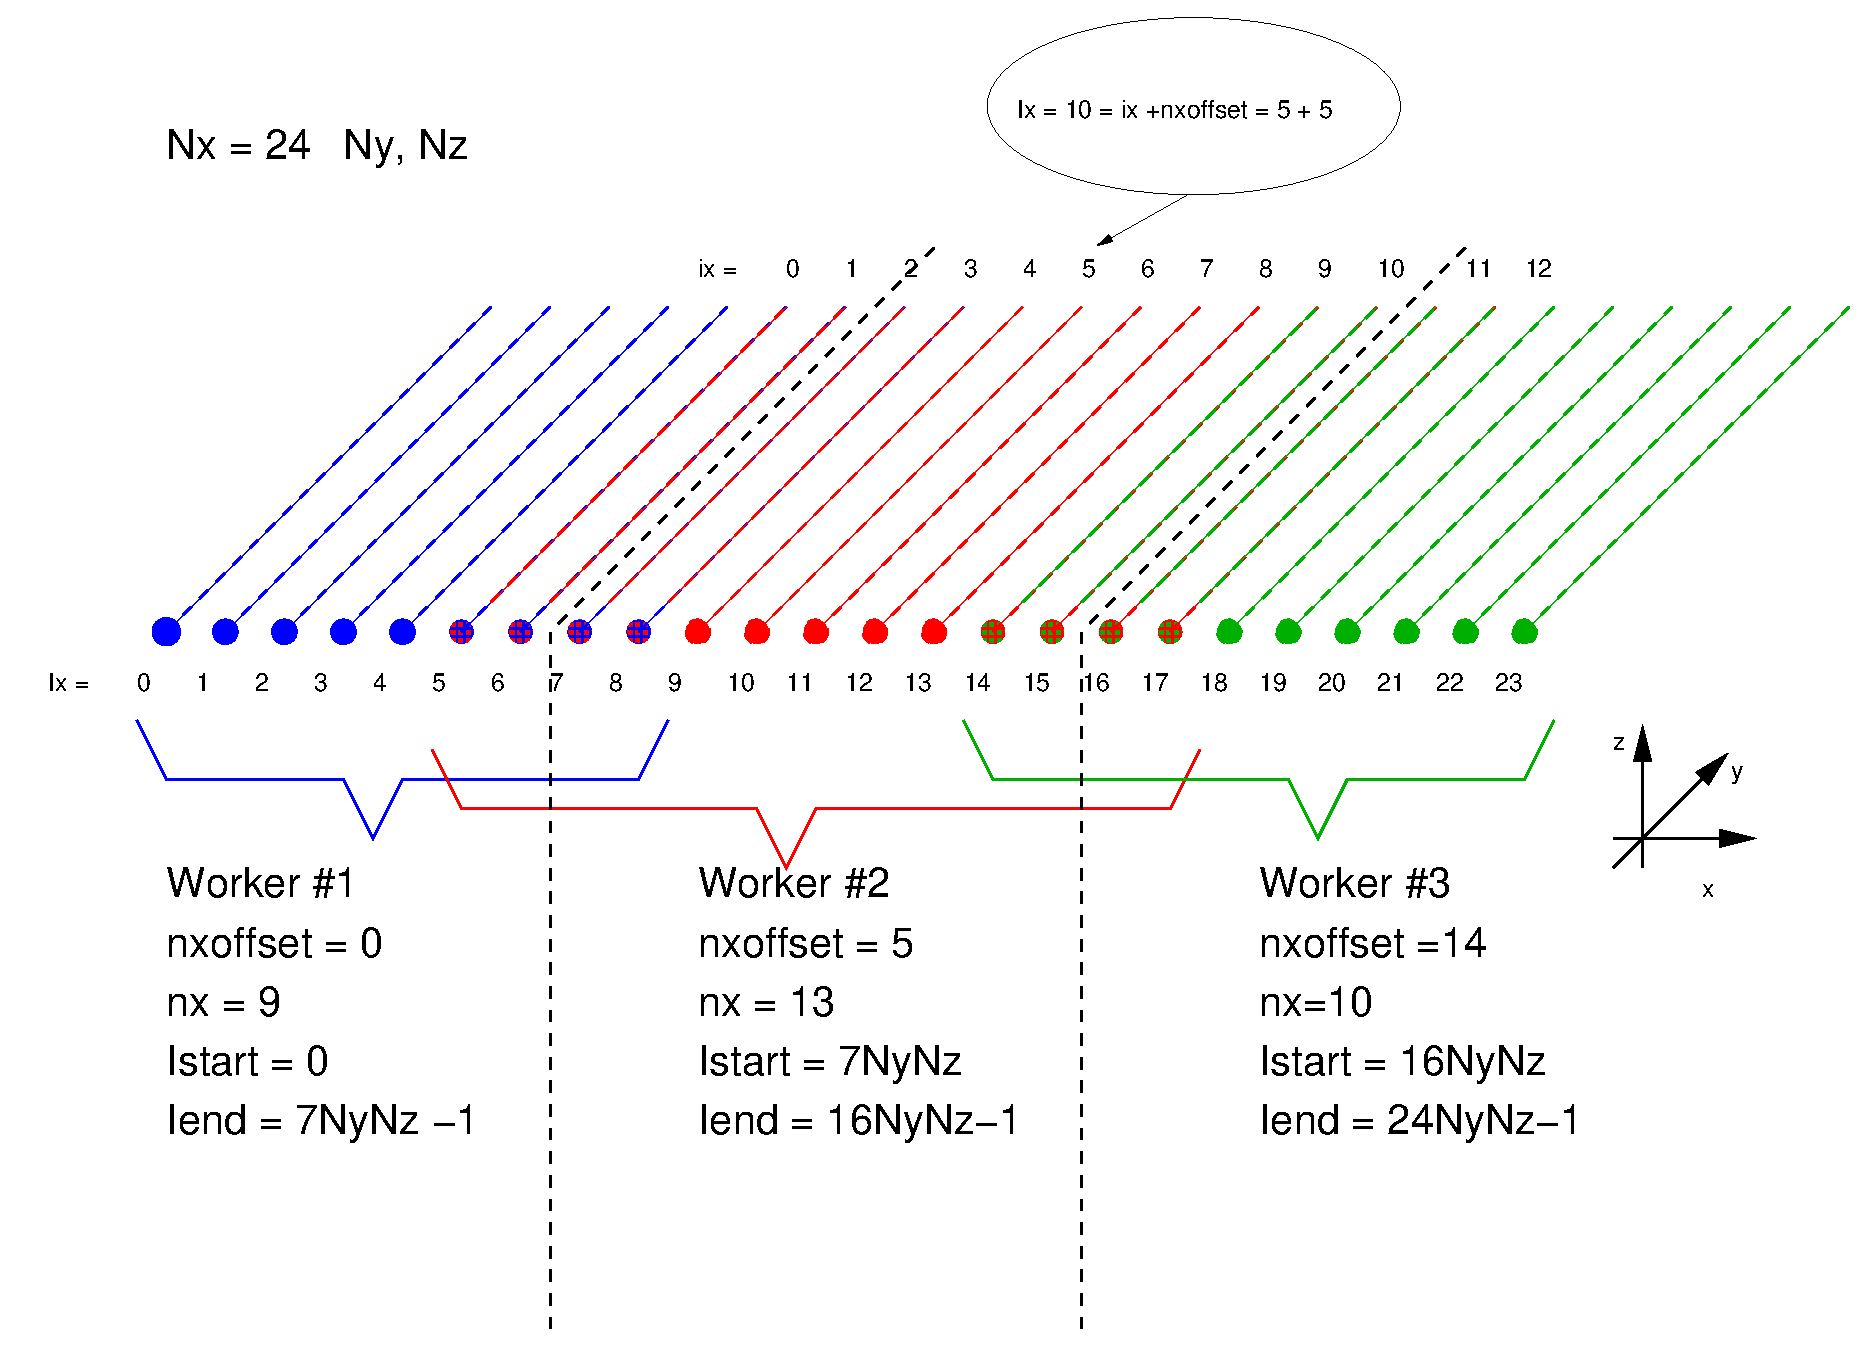
\includegraphics[angle=0,width=\textwidth]{\figuredir/domainDecomp.eps}
  \end{center}
  \caption{Domain decomposition, here for an example with three
    SnowDriftWorkers and $N_x=24$. Only the bottom layer of nodes of
    the whole simulation domain in the $xy$ plane is shown. Some
    examples values of the variables used in the code are shown.}
\end{figure}
The overlap (or ghost nodes) between adjacent domains is determined by
PopC and contains two layers of nodes. Thus, the global $N_x$ is not
simply the sum over the local $n_x$ due to the overlap.

For the present decomposition it is advantageous to use a node
enumeration such that consecutive blocks of node-numbers are hold by
one processor. This leads to a global node enumeration as shown in
Fig.\ \ref{globalNode}: The global mapping of a node with global
coordinates $I_x,I_y,I_z$ onto an global node index $I$ is given by
$I=I_xN_zN_y+I_zN_y+I_y$, i.e. the lattice is traversed along
coordinate directions in the order $y,z,x$. Global node indices for an
element with local element number are available on each processor via
the \verb+globalNodeMap+ array which is defined in
\verb+SnowDriftWorker.cc+ It maps the node numbers $\in\{0,1..8\}$
within an element with local element number
$\in\{0,1..(n_x-1)(n_y-1)(n_z-1)-1\}$ to the global node index which
is e.g. $\in\{5N_yN_z,..18N_yN_z-1\}$ for Worker no 2 in the three
processor example given above. Note, that the elements are enumerated
by traversing the lattice in along coordinate directions in the order
$x,y,z$.

In contrast, locally the nodes are enmuerated also in the
$x,y,z$-scheme which was the old enumeration scheme and which was left
for data structure which survived in the present parallel
implementation (i.e. the \verb+nodes+-array). More precisely the
enumeration is according to $i=i_x+i_yn_x+i_zn_yn_x$ for a node with
local coordinates $i_x,i_y,i_z$ and local index $i$. The
\verb+nodeMap+-array is defined in \verb+SnowDrift.cc+ such that node
numbers $\in\{0,1..8\}$ within an element with a local element number
$\in\{0,1..(n_x-1)(n_y-1)(n_z-1)-1\}$ is mapped onto the the local
node index $\in\{0,1..n_xn_yn_z-1\}$. Again, the elements
are enumerated in the $x,y,z$-scheme.

\begin{figure}[t]
  \begin{minipage}[c]{0.48\textwidth}
      \includegraphics[angle=0,width=7cm]{\figuredir/globalNodeEnumeration.eps}
      \caption{Global node enumeration on the example of Worker 2 from
        the domain decomposition in Fig.\ \ref{decomp}}
    \label{globalNode}
  \end{minipage}
  \hfill
  \begin{minipage}[c]{0.48\textwidth}
    \includegraphics[angle=0,width=7cm]{\figuredir/localNodeEnumeration.eps}
    \caption{Local node enumeration on the example of Worker 2 from
      the domain decomposition in Fig.\ \ref{decomp}}
    \label{localNode}
  \end{minipage}
\end{figure}


% ------------------------------------------------------------
\subsubsection{Communication}
% ------------------------------------------------------------
During the assembling and the solution of the linear system the
communication is automatically done by PETSc. The values of the
solution vector on the processor domain boundary are afterwards
distributed to neighboring processors by POPC++ in the
\verb+ExchangeBoundSuspension+ method in \verb+SnowDriftWorker.cc+.
This is necessary to compute the deposition flux in
\verb+SnowDriftFEControl.cc+ consistently.


% ------------------------------------------------------------
% ------------------------------------------------------------
\subsection{Problems with the present parallel drift}
% ------------------------------------------------------------
% ------------------------------------------------------------

% ------------------------------------------------------------
\subsubsection{No unifying source code for sequential and parallel mode}
% ------------------------------------------------------------
The main problem of the present parallel implementation is that it
cannot be run sequentially. To explain this difficulty it is necessary
to understand the following details of the implementation: Every
MPI/PETSc program requires the initialization of the parallel
communicator via \verb+PetscInitialize()+ which in turn calls
\verb+MPI_Init()+. This is implicitely done by POPC++ during
construction of the SnowDriftWorkers. This implies i) all PETSc
variables (vectors,matrices) have to be members of the
\verb+SnowDriftWorker+-class and ii) all workers are automatically
ready to execute MPI/PETSc code.

This reveals the two problems when one wants to take over this
implementation to a sequential mode: Presently, in sequential mode no
workers are constructed. Consequently i) no PETSc variables are
available at all ii) and no call to \verb+PetscInitialize()+ is done.

A workaround might be possible by (a lot of?) conditional compilation:
First, in sequential mode \verb+PetscInitialize()+ must be invoked
manually somewhere else (where? probably in AlpineMain). Second, in
sequential mode all PETSc variables must be members of the class
\verb+SnowDrift+ and {\em not} members of the class
\verb+SnowDriftWorker+. Vice versa in parallel mode.

Therefore, the parallel version is included in an additional directory
\verb+snowdrift_par+ in the repository.


% ------------------------------------------------------------
\subsubsection{Dynamic library completion}
% ------------------------------------------------------------
It is necessary to additionally hack the snowdriftworker.module after
running \verb+make deploy_par+ in order to appropriately include the
dynamic libraries. This is achieved by the helper application
\verb+parocexe+ which is located in the \verb+tools+ directory located
in your \verb+trunk+ directory. The call to parocexe is included in
the \verb+Makefile.par+.


% ------------------------------------------------------------
% ------------------------------------------------------------
\subsection{If you want to use it}
% ------------------------------------------------------------
% ------------------------------------------------------------
\begin{enumerate}
\item adjust your environment:
  \verb+source ./tools/popc-petsc.env+
\item \verb+make all_par -f Makefile.par+ 
\item \verb+make deploy_par -f Makefile.par+
\item \verb+./sc_drift_par.sh+
\end{enumerate}

With the present ``installation'' of popc only the MPI processes are
computed in parallel, the remaining modules are running on your local
machine.


% ------------------------------------------------------------
% ------------------------------------------------------------
\section{TODO}
% ------------------------------------------------------------
% ------------------------------------------------------------
\begin{enumerate}
\item install a proper version of popc-1.1 in /usr/local against mpi
  (should be the version \verb+/usr/local/mpich-1.2.5.2+ since
  petsc-2.3.0 is compiled against it) and \verb+petsc-2.3.0-popc+
\end{enumerate}



%%%%%%%%%%%%%%%%%%%%%%%%%%%%%%%%%%%%%%%%%%%%%%%%%%%%%%%%%%%%%%%%%%
%%%%%%%%%%%%%%%%%%%%%%%%%%%%%%%%%%%%%%%%%%%%%%%%%%%%%%%%%%%%%%%%%%
% ------------------------------------------------------------
\chapter{Data Assimilation Module}\label{ch:assimilation}
% ------------------------------------------------------------
%%%%%%%%%%%%%%%%%%%%%%%%%%%%%%%%%%%%%%%%%%%%%%%%%%%%%%%%%%%%%%%%%%
%%%%%%%%%%%%%%%%%%%%%%%%%%%%%%%%%%%%%%%%%%%%%%%%%%%%%%%%%%%%%%%%%%

%%%%%%%%%%%%%%%%%%%%%%%%%%%%%%%%%%%%%%%%%%%%%%%%%%%%%%%%%%%%%%%%%%
% ------------------------------------------------------------
\section{Files}
% ------------------------------------------------------------
%%%%%%%%%%%%%%%%%%%%%%%%%%%%%%%%%%%%%%%%%%%%%%%%%%%%%%%%%%%%%%%%%%
The data assimilation module in \verb+./assimilation+
contains the files 
\begin{verbatim}
  DataAssimilation.h
  DataAssimilation.ph
  DataAssimilation.cc
  PackDataAssimilation.cc
\end{verbatim}


%%%%%%%%%%%%%%%%%%%%%%%%%%%%%%%%%%%%%%%%%%%%%%%%%%%%%%%%%%%%%%%%%%
% ------------------------------------------------------------
\section{Description}
% ------------------------------------------------------------
%%%%%%%%%%%%%%%%%%%%%%%%%%%%%%%%%%%%%%%%%%%%%%%%%%%%%%%%%%%%%%%%%%

The assimilation module (often abbreviated by ``DA'' or ``da'' in the
code) is responsible for any data assimilation specific computations.
Presently, it basically hosts memory for the assimilation data which
could have been included also in some of the other modules since only
direct insertion like assimilation without any computation is
implemented. It has been decided to add an additional module though
for the sake of generality since for more sophisticated assimilation
schemes (like a Kalman Filter) extensive numerics might be required
(i.e. for the computation of the Kalman gain matrix).

The module can be enabled by the switch \verb+-enable-da+ in the
command line options of Alpine3d limilar to the other modules.
Additionally, a path to the assimilation data has to be provided 
by adding the switch

\verb+-dadir=<path to da-data, without terminating slash>+

Having enabled the data assimilation the basic working steps of
Alpine3d which involve the assimilation are given below:

\begin{enumerate}
\item At each time step the \verb+Compute()+ method of the
  DataAssimlation class is invoked in \verb+AlpineControl::Run+ in
  \verb+AlpineControl.cc+ which forces its input member to try to read
  assimilation data from the specified directory \verb+dadir+. In that
  directory, the program expects data in files with names
  \verb+<YYYYMMDDHH>.sca+ which must contain integer data and should
  be formatted according to the usual Ascii ArcInfo grid format.
\item If data is available in that directory with the correct
  timestamp it is read into the memory of the assimilation class and
  send to snowpack, which itself distributes the data to its workers
  (if run in parallel). If no DA-data is available at that timestep an
  exception is thrown and everything continues regularly.
\item Within snowpack, \verb+Snowpack::Assimlate()+ is invoked and the
  DA data is used to control actions in Snowpack. For the present
  example in the case of SCA data cf \verb+Snowpack::Assimilate()+ in
  \verb+SnowInterface.cc+ for the details of the actions.
\end{enumerate}



%%%%%%%%%%%%%%%%%%%%%%%%%%%%%%%%%%%%%%%%%%%%%%%%%%%%%%%%%%%%%%%%%%
% ------------------------------------------------------------
\section{Modifications in other modules}
% ------------------------------------------------------------
%%%%%%%%%%%%%%%%%%%%%%%%%%%%%%%%%%%%%%%%%%%%%%%%%%%%%%%%%%%%%%%%%%
The modification in other files which were necessary to build in a new
class (parclass) are listed below:
\begin{itemize}
\item  add ./assimlation directory
\item modify all Makefiles (for obvious reasons)
\item in ./main (creating the DA module in AlpineControl)
\item in ./common (add new exceptions, etc)
\item in ./snowpack: add pointer to assimilation module, add
  assimilation routines, add distribution of DA data to workers
\item in ./inout: add a method for reading DA-data and a method for
  getting the grid dimensions (GetGridSize(...))
\end{itemize}

%%%%%%%%%%%%%%%%%%%%%%%%%%%%%%%%%%%%%%%%%%%%%%%%%%%%%%%%%%%%%%%%%%
%%%%%%%%%%%%%%%%%%%%%%%%%%%%%%%%%%%%%%%%%%%%%%%%%%%%%%%%%%%%%%%%%%
\begin{thebibliography}{99}
%%%%%%%%%%%%%%%%%%%%%%%%%%%%%%%%%%%%%%%%%%%%%%%%%%%%%%%%%%%%%%%%%%
%%%%%%%%%%%%%%%%%%%%%%%%%%%%%%%%%%%%%%%%%%%%%%%%%%%%%%%%%%%%%%%%%%
\bibitem{popc}
  See documentation on \\
  (\verb+http://gridgroup.tic.hefr.ch/popc/index.php/Main_Page+)
  
\bibitem{lehning_2006}
    Lehning, M., V\"olksch, I., Gustafsson, D., Nguyen, T.A., St\"ahli, M.,
    Zappa, M., (2006)
    ALPINE3D: A detailed model of mountain surface processes and its
    application to snow hydrology,
    \textit{Hydrol. Processes, 20}, 2111-2128.

\bibitem{petsc}
  See documentation on \\
  (\verb+http://www-unix.mcs.anl.gov/petsc/petsc-as/+)

\bibitem{ryser_2004}
  Ryser, M.
  Numerical Simulation of Snow Transport Above Alpine Terrain
  Internship Report
  see \verb+MarcRyser_Drift_Final.pdf+

\bibitem{gt}
  See documentation on \\
  (\verb+http://www.globus.org/toolkit/+)

\bibitem{svn}
  Online book on\\
  (\verb+http://svnbook.red-bean.com+)

\bibitem{jon07}
  Jonas, T. (SLF)
  ``Alpine3d Crash Course for the Snow Hydrology Research Group''
  
\end{thebibliography}





\end{document}
